\documentclass[a4paper,12pt]{article}
\usepackage[spanish]{babel}
\hyphenation{co-rres-pon-dien-te}
\usepackage[utf8]{inputenc}
\usepackage[T1]{fontenc}
\usepackage{graphicx}
\usepackage[pdftex,colorlinks=true, pdfstartview=FitH, linkcolor=blue,
citecolor=blue, urlcolor=blue, pdfpagemode=UseOutlines, pdfauthor={H. Asorey},
pdftitle={F3B - Guía 02}]{hyperref}
\usepackage[adobe-utopia]{mathdesign}

\hoffset -1.23cm
\textwidth 16.5cm
\voffset -3.5cm
\textheight 26.5cm

%----------------------------------------------------------------
\begin{document}
\title{
{\normalsize{Universidad Nacional de Río Negro - Profesorado de Física}}\\
Física IIIB 2022 \\ Guía 02: Primer Principio
}
\author{Asorey}
\date{31 de Marzo de 2022}
\maketitle

\begin{enumerate}
	\setcounter{enumi}{21}      %% esta guia va del problema 01 al 06

    \item {\bf{Tres cilindros}}

        Tres pistones cilindros idénticos contienen $1$\,mol de un gas ideal 
        monoatómico, biatómico y triatómico respectivamente. Todos los gases se
        encuentran inicialmente en CNPT. Si al gas contenido en cada pistón se
        le entregan $13.2$\,kJ en forma de calor de manera que la presión se
        mantiene constante, calcule el volumen final de cada recipiente.
        ¿Qué tipo de gas usaría si tuviera que hacer un elevador utilizando 
        estos pistones? Justifique en el marco de la teoría cinética de los
        gases los resultados obtenidos.
		\\{\bf{R}}: $V_i=0,0224$\,m$^3$; $V_{f,\mathrm{mono}}=0,0745$\,m$^3$;
		$V_{f,\mathrm{bi}}=0,0596$\,m$^3$; $V_{f,\mathrm{tri}}=0,055$\,m$^3$;

	\item {\bf{Diferencias}}
		
		Tres pistones cilíndricos idénticos de radio $r=0.2$\,m contienen cada
		uno 10\,mol de un gas ideal monoatómico a $T=1000$\,K y $p=20$\,atm.
		El gas del primer pistón es sometido a una expansión isobárica, el del
		segundo a una expansión isotérmica y el del tercer cilindro a una
		expansión adiabática. En todos los casos el volumen final es el doble
		del volumen inicial. Calcule: a) Los volúmenes iniciales y finales en
		cada pistón. b) Calcule el trabajo realizado por el gas y la altura
		inicial y final de cada pistón. c) Cuando corresponda calcule para cada
		proceso: la cantidad de calor suministrada, las temperaturas iniciales
		y finales, y la variación en la energía interna del gas.
		\\{\bf{R}}: a) son iguales para todos, $V_i=0,04103$\,m$^3$ y
		$V_{f}=0,08206$\,m$^3$; b) las alturas son iguales para todos los
		pistones $h_i=0,327$\,m y $h_f=0,653$\,m. Los trabajos serán
		$W_1=83,15$\,kJ; $W_2=57,6$\,kJ; y $W_3=46,1$\,kJ; c) $\Delta
		U_1=124,7$\,kJ y $Q_1=208,85$\,kJ; $\Delta U_2=0$ y $Q_2=57,6$\,kJ;
		$\Delta U_3=-46,1$\,kJ y $Q_3=0$;  
	
	\item {\bf{Transformaciones}}
		
		Un mol de un gas ideal a presión $P_A$ ocupa un volumen $V_A$. Se lo
		calienta en una transformación isócora entregándole una cantidad de
		calor $Q_{1}$ hasta que el sistema alcanza la presión
		$P_B$. Luego se vuelve a calentarlo, entregándole una cantidad de calor
		$Q_2 = Q_1$, pero mediante una
		transformación isobárica hasta alcanzar un volumen $V_C$. 
		\begin{enumerate}
			\item En un diagrama $P-V$, dibuje las transformaciones que el gas
				realiza, identificando las curvas isotermas asociadas a cada
				estado. ¿Es un ciclo? ¿Por qué?
			\item Obtenga una expresión del cociente entre los calores
				específicos $C_P$ y $C_V$ como función de las temperaturas
				de los estados.
			\item A partir del valor del cociente de los calores específicos
				para un gas ideal monoatómico, $C_P / C_V = \gamma = 5/3$, y
				sabiendo que inicialmente el gas se encontraba en CNPT y que la
				presión final es el doble de la presión inicial, calcule:
				\begin{enumerate}
					\item El volumen inicial $V_A$ y final $V_C$
					\item La presión final $P_C$
					\item Las temperaturas $T_B$ y $T_C$. 
					\item La cantidad de calor total suministrada.
				\end{enumerate}
		\end{enumerate}
		{\bf{R}}: b) $\gamma = \frac{C_P}{C_V} = \frac{T_B-T_A}{T_C-T_B}$; c1)
		$V_A=V_B=0,0224$\,m$^3$, $V_C=0,0291$\,m$^3$; c2) $P_C=P_B=202650$\,Pa;
		c3) $T_A=273$\,K, $T_B=546$\,K, $T_C=709,8$\,K; c4)
		$Q_1=Q_2=3404,5$\,J.
		
	\item {\bf{Caldera}}
		
		En el recipiente de presión de una caldera hay una temperatura de
		230\,$^\mathrm{o}$C y una presión constante de 30\,bar. En cada ciclo
		de trabajo el vapor desplaza un pistón con una superficie de
		$0.2$\,m$^2$ una distancia de $0.4$\,m. a) ¿Cuánto vale el trabajo
		entregado en cada ciclo? b) ¿Cuál es la potencia entregada por la
		máquina de vapor cuando se desarrollan 600 ciclos de trabajo por
		minuto?
		\\{\bf{R}}: a) $W=240$\,kJ; b) La potencia erogada es $P=2,4$\,MW.
	
	\item {\bf{Un ciclo para no perder la costumbre}}
		
		Una máquina térmica utiliza como fluido un gas ideal monoatómico, y
		funciona con dos fuentes a temperaturas $T_A = 297$\,K y $T_B =
		990$\,K. El ciclo consiste en un calentamiento isocórico, seguido por
		una expansión isotérmica, para terminar con una compresión isobárica.
		El volumen inicial es $V_A=0.1$\,m$^3$ a una presión de
		$P_A=101325$\,Pa.
		
		\begin{enumerate}
			\item Dibuje el ciclo en un diagrama P-V.
			\item Completar el cuadro de estados 
			\item Completar el cuadro de transformaciones
			\item Hallar el rendimiento $\eta$ del ciclo, y compararlo con el
				rendimiento del ciclo de Carnot funcionando entre esas mismas
				temperaturas.
			\item Si el motor opera a un régimen de $3000$ ciclos por segundo,
				calcule la potencia del motor y la cantidad de calor entregada
				por segundo a la fuente fría.
		\end{enumerate}
		{\bf{R}}: b) $P_A=101325$\,Pa, $V_A=0,1$\,m$^3$, $n_A=4,1035$\,mol,
		$T_A=297$\,K; $P_B=337750$\,Pa, $V_B=0,1$\,m$^3$, $n_B=4,1035$\,mol,
		$T_B=990$\,K; $P_C=101325$\,Pa, $V_C=0,33$\,m$^3$, $n_C=4,1035$\,mol,
		$T_C=990$\,K; c) $Q_1=35463,8$\,J, $\Delta U_1=35463,8$\,J, $W_1=0$;
		$Q_2=40664,2$\,J, $\Delta U_2=0$\,J, $W_2=40664,2$\,J;
		$Q_3=-59106,3$\,J, $\Delta U_3=-35463,8$\,J, $W_3=-23642,5$\,J; d)
		$\eta=17021,7/76127,9 = 0,2236 = 22,36\%$; $\eta_{\mathrm{Carnot}} =
		0,7 = 70\%$; e) Potencia $P=51,06$\,MW,
		$Q_{\mathrm{fria}}=Q_3=-177,32$\,MJ cada segundo.
	
	\item {\bf{El cuadrado}}
		
		Una máquina térmica está equipada con $n=1000$\,moles de un gas ideal
		di-atómico, inicialmente en CNPT, que opera con el siguiente ciclo: 1)
		calentamiento isocórico hasta quintuplicar la temperatura inicial; 2)
		expansión isobárica hasta quintuplicar el volumen inicial; 3)
		enfriamiento isocórico; 4) compresión isobárica.
		
		\begin{enumerate}
			\item Complete el cuadro de estados, encontrando los valores de
				$P$, $V$, $T$ y $n$ para cada uno de los estados $A$, $B$, $C$
				y $D$. 
			\item En el diagrama $P-V$ ubique los estados y dibuje las
				transformaciones experimentadas por el gas.
			\item Complete el cuadro de transformaciones, encontrado los
				cambios de energía interna, calor y trabajo en cada
				transformación.
			\item Calcule el rendimiento de la máquina y compárelo con el
				rendimiento del ciclo de Carnot equivalente (aquel que funciona
				con las mismas fuentes térmicas).
		\end{enumerate}
		{\bf{R}}: a) $P_A=101325$\,Pa, $V_A=22,4$\,m$^3$, $n_A=1000$\,mol,
		$T_A=273$\,K; $P_B=506634,4$\,Pa, $V_B=22,4$\,m$^3$, $n_B=1000$\,mol,
		$T_B=1365$\,K; $P_C=506634,4$\,Pa, $V_C=112$\,m$^3$, $n_C=1000$\,mol,
		$T_C=6825$\,K; $P_D=101325$\,Pa, $V_D=112$\,m$^3$, $n_D=1000$\,mol,
		$T_D=1365$\,K; c) $Q_1=22,7$\,MJ, $\Delta U_1=22,7$\,MJ, $W_1=0$;
		$Q_2=158,9$\,MJ, $\Delta U_2=113,5$\,MJ, $W_2=45,4$\,MJ;
		$Q_3=-113,5$\,MJ, $\Delta U_3=-113,5$\,MJ, $W_3=0$; $Q_4=-31,8$\,MJ,
		$\Delta U_4=-22,7$\,MJ, $W_4=-9,1$\,MJ; d) $\eta=36,3/181,6 = 0,2 =
		20\%$; $\eta_{\mathrm{Carnot}} = 0,96 = 96\%$;

	\item {\bf{Carnot}}

		Una máquina térmica funciona con $n=0,2$\,mol de un gas ideal biatómico
		siguiendo un ciclo de Carnot entre las temperaturas
		$T_{\mathrm{caliente}}=500$\,K y $T_{\mathrm{fria}}=300$\,K. La presión
		del estado inicial es $P_A=10^6$\,Pa y luego de la primera expansión
		isotérmica el volumen se duplica, es decir, $V_B = 2 V_A$.
		\begin{enumerate}
			\item Complete el cuadro de estados, encontrando los valores de
				$P$, $V$, $T$ y $n$ para cada uno de los estados $A$, $B$, $C$
				y $D$. 
			\item En el diagrama $P-V$ ubique los estados y dibuje, en escala,
				las transformaciones experimentadas por el gas.
			\item Complete el cuadro de transformaciones, encontrado los
				cambios de energía interna, calor y trabajo en cada
				transformación.
			\item Calcule el eficiencia de la máquina a partir de la definición
				$\eta=W_{\mathrm{neto}} / Q_{>0}$ y compárelo con el obtenido
				utilizando la fórmula del rendimiento de la máquina de Carnot. 
		\end{enumerate}
		{\bf{R}}: a) 
		$P_A=10^6$\,Pa, $V_A=8,31\times10^{-4}$\,m$^3$, $n_A=0,2$\,mol,
		$T_A=500$\,K; $P_B=5\times 10^5$\,Pa, $V_B=16,63\times10^{-4}$\,m$^3$,
		$n_B=0,2$\,mol, $T_B=500$\,K; $P_C=83656,4$\,Pa,
		$V_C=59,63\times10^{-4}$\,m$^3$, $n_C=0,2$\,mol, $T_C=300$\,K;
		$P_D=167312,9$\,Pa, $V_D=29,81\times10^{-4}$\,m$^3$, $n_D=0,2$\,mol,
		$T_D=300$\,K; c) $Q_1=576,3$\,J, $\Delta U_1=0$, $W_1=576,3$\,J;
		$Q_2=0$, $\Delta U_2=-831,4$\,J, $W_2=831,4$\,J; $Q_3=-345,8$\,J,
		$\Delta U_3=0$, $W_3=-345,8$\,J; $Q_4=0$, $\Delta U_4=831,4$\,J,
		$W_4=-831,4$\,J; d) $\eta=230,5/576,3 = 0,4 = 40\%$;
		$\eta_{\mathrm{Carnot}} = 0,4 = 40\%$.

	\item {\bf{Carnot, con números}}

		Una máquina térmica opera siguiendo un ciclo de Carnot erogando una
		potencia de $3$\,MW con un rendimiento del 75\%.  Contiene $100$\,moles de
		un gas ideal triatómico, y está instalada cerca de un río a temperatura
		$T_C=280$\,K. La puesta en marcha se realiza calentando al gas desde
		CNPT en forma isocórica hasta alcanzar la temperatura de trabajo.
		\begin{enumerate}
			\item Dibuje el ciclo en un diagrama P-V.
			\item Complete el cuadro de estados y el cuadro de transformaciones.
		\end{enumerate}
		{\bf{R}}:  
		$P_A=415700$\,Pa, $V_A=2,24$\,m$^3$, $n_A=100$\,mol, $T_A=1120$\,K; 
		$P_B=5665$\,Pa, $V_B=164,38$\,m$^3$, $n_B=100$\,mol, $T_B=1120$\,K; 
		$P_C=22,1$\,Pa, $V_C=10520,32$\,m$^3$, $n_C=100$\,mol, $T_C=280$\,K; 
		$P_D=1623,83$\,Pa, $V_D=143,36$\,m$^3$, $n_D=100$\,mol, $T_D=280$\,K; 
		$Q_1=4$\,MJ, $\Delta U_1=0$, $W_1=4$\,MJ;
		$Q_2=0$, $\Delta U_2=-2,095$\,MJ, $W_2=2,095$\,MJ;
		$Q_3=-1$\,MJ, $\Delta U_3=0$, $W_3=-1$\,MJ;
		$Q_4=0$, $\Delta U_4=+2,095$\,MJ, $W_4=-2,095$\,MJ;
		$\eta=3/4 = 0,75 = 75\%$; $\eta_{\mathrm{Carnot}} = 0,75 = 75\%$.
	
	\item {\bf{Máquina de Carnot directa y reversa}}
		
		Suponga una máquina térmica que funciona mediante un ciclo de Carnot
		entre dos fuentes a temperaturas $T_A=700$\,K y $T_C=300$\,K y utiliza
		como fluido un gas ideal di-atómico. Al iniciar el ciclo, el gas se
		encuentra a la temperatura $T_A$, una presión de $10$\,hPa y ocupa un
		volumen de $0.007$\,m$^3$. Al finalizar el primer tramo del ciclo la
		presión del gas desciende a $P_B=8$\,hPa.
		\begin{enumerate}
			\item Dibuje el ciclo en un diagrama P-V.
			\item Complete el cuadro de estados y el cuadro de transformaciones
			\item Halle el rendimiento total el ciclo, y compruebe si coincide
				con el valor esperado para un ciclo de Carnot.
			\item ¿Dependerá el rendimiento de la atomicidad del gas? ¿y la
				cantidad total de trabajo obtenida?
			\item Calcule la potencia entregada por la máquina sabiendo que la
				misma puede funcionar a 210 ciclos por segundo.
			\item Invierta el ciclo y calcule el trabajo que es necesario
				entregar a la máquina térmica para hacerla funcionar en el
				sentido inverso.
		\end{enumerate}
		{\bf{R}}: 
		b)
		$P_A=1000$\,Pa, $V_A=0,007$\,m$^3$, $n_A=0,001203$\,mol, $T_A=700$\,K; 
		$P_B=800$\,Pa, $V_B=0,00875$\,m$^3$, $n_B=0,001203$\,mol, $T_B=700$\,K; 
		$P_C=41,23$\,Pa, $V_C=0,0728$\,m$^3$, $n_C=0,001203$\,mol, $T_C=300$\,K; 
		$P_D=51,53$\,Pa, $V_D=0,0582$\,m$^3$, $n_D=0,001203$\,mol, $T_D=300$\,K; 
		$Q_1=1,56$\,J, $\Delta U_1=0$, $W_1=1,56$\,J;
		$Q_2=0$, $\Delta U_2=-10$\,J, $W_2=10$\,J;
		$Q_3=-0,67$\,J, $\Delta U_3=0$, $W_3=-0,67$\,J;
		$Q_4=0$, $\Delta U_4=10$\,J, $W_4=-10$\,J;
		c)
		$\eta=3/4 = 0,571 = 57,1\%$; $\eta_{\mathrm{Carnot}} = 0,571 = 57,1\%$.
		d) trabajo individual.
		e) Potencia$=187,4$\,W.
		f) Dado que la máquina de Carnot es reversible: funcionamiento directo,
		$W_{\mathrm{neto}}=0,89$\,J; funcionamiento inverso, $W_{\mathrm{neto}}=-0,89$\,J.
	
	\item {\bf{Auto 1: rendimiento}}\label{auto1}
		
		Para alcanzar una velocidad máxima de 150\,km/h se requiere toda la
		potencia de un motor de automóvil de 100\,kW. ¿Cuánta nafta se requiere
		para recorrer 100\,km cuando el motor tiene un eficiencia de 25\%?
		Discutir el balance energético total. Equivalente energético de la
		nafta: 12 kWh/kg.
		\\{\bf{R}}: Se consumen $22,22$\,kg de nafta.
	
	\item {\bf{Energía del mar}}
		
		Se quiere usar la diferencia de temperatura entre la superficie del
		agua de mar de 25\,$^\mathrm{o}$C y de las capas profundas de
		4\,$^\mathrm{o}$C para producir energía eléctrica.
		\begin{enumerate}
			\item ¿Cuál es la eficiencia termodinámica máxima que esperaría
				encontrar con este método de producción de energía?
			\item ¿Cuántos m$^3$ de agua por segundo se necesitaría para
				erogar una potencia de 1 GW de trabajo neto (eléctrico)?
		\end{enumerate}
		{\bf{R}}: a) $\eta=0,07 = 7\%$; b) se requieren $162,51$\,m$^3$/s
		(caudal del Río Limay = $700$\,m$^3$/s). 

	\item {\bf{Horno solar}}
		
		Un diseño de horno solar permite calentar agua hasta
		90$^\mathrm{o}$\,C. Una persona propone usar esta agua caliente para
		hacer funcionar una máquina térmica. a) ¿Qué eficiencia se podría alcanzar
		para esa máquina si la temperatura ambiente es de 20$^\mathrm{o}$\,C?
		b) Si la constante solar es de $1400$\,W\,m$^{-2}$ y la absorción atmosférica
		en nuestras latitudes es del $50\%$, ¿cuál es el área que debe tener el
		colector solar para calentar $1$\,kg de agua desde temperatura ambiente
		hasta la temperatura máxima en $1$\,minuto?
		\\{\bf{R}}: a) $\eta=0,193 = 19,3\%$; b) Debe tener un área de
		$7$\,m$^2$. 
	
	\item {\bf{Máquina térmica}}
		
		Una máquina térmica tiene una eficiencia del 30\% y eroga $3$\,GW de
		potencia mecánica.
		\begin{enumerate}
			\item En un segundo, ¿qué cantidad de calor recibe de la fuente
				caliente? ¿Qué cantidad de calor entrega al medio ambiente?
			\item Este calor debe ser entregado a un río cuya temperatura no
				debe subir más de 2$^\mathrm{o}$\,C. ¿Qué caudal mínimo (en
				m$^3$ s$^{-1}$) debe tener ese río?
		\end{enumerate}
		{\bf{R}}: a) $Q_{\mathrm{Abs}}=10$\,GJ; $Q_{\mathrm{Ent}}=7$\,GJ; b) se
		requieren $836,12$\,m$^3$/s (caudal del Río Negro = $1014$\,m$^3$/s). 
	
	\item {\bf{Trigo}}
		
		El valor nutritivo del trigo que se produce en un metro cuadrado de
		tierra fértil es de $2$\,kWh. Si en esa región agrícola la irradiancia solar
		durante el verano es $\sim 700$\,W\,m$^{-2}$ durante unas 7 horas
		diarias en promedio y que el trigo demora cinco meses en madurar.  
		¿Cual es el rendimiento energético del trigo? 
		\\{\bf{R}}: a) $\eta=2/735=0,00272 = 0,272\%$;

	\item {\bf{Auto 2: ciclo Otto}}
		
		El ciclo Otto opera en los motores de autos que funcionan con nafta
		(gasolina) como combustible. Es usual hablar del ciclo de cuatro etapas
		(Admisión, Compresión, Explosión y Escape), aunque en realidad son seis
		las etapas que experimenta la mezcla de combustible y aire: 1)
		expansión de la mezcla a presión constante (admisión, $n$ aumenta); 2)
		compresión adiabática (compresión); 3) calentamiento isócoro
		(combustión); 4) expansión adiabática (explosión+expansión); 5)
		enfriamiento isócoro; 6) compresión isóbara (escape, $n$ disminuye).
		Descartando las etapas 1 y 6, donde hay cambio en la cantidad de gas,
		suponiendo que durante las etapas 2, 3, 4 y 5 la cantidad de mezcla es
		$n=0,02$\,mol (valor aproximado para un motor de $2000$\,cm$^3$), y
		utilizando los valores del diagrama PV visto en clase, realice los
		siguientes ejercicios:
		\begin{enumerate}
			\item Complete el cuadro de estados $A$, $B$, $C$ y $D$. 
			\item Complete el cuadro de las transformaciones $2$, $3$, $4$ y
				$5$.  
			\item El rendimiento termodinámico del motor. Compárelo con el
				rendimiento de un ciclo de Carnot equivalente y con el dato de
				la eficiencia de un motor a combustión interna del problema
				\ref{auto1}.
			\item Si el motor funciona en régimen a $3600$\,RPM, calcule la
				cantidad de calor producida por el consumo de combustible, el
				trabajo neto liberado y la cantidad de calor liberada en la
				atmósfera cada hora de funcionamiento.		
		\end{enumerate}
		{\bf{R}}: 
		b)
		$P_A=101325$\,Pa, $V_A=0,00048$\,m$^3$, $n_A=0,02$\,mol, $T_A=293$\,K; 
		$P_B=1874512,5$\,Pa, $V_B=0,00006$\,m$^3$, $n_B=0,02$\,mol, $T_B=676$\,K; 
		$P_C=5015587,5$\,Pa, $V_C=0,00006$\,m$^3$, $n_C=0,02$\,mol, $T_C=1810$\,K; 
		$P_D=253312,5$\,Pa, $V_D=0,00048$\,m$^3$, $n_D=0,02$\,mol, $T_D=731$\,K;
		$Q_2=0$, $\Delta U_2=159,6$\,J, $W_2=-159,6$\,J;
		$Q_3=471,2$\,J, $\Delta U_3=471,2$\,J, $W_3=0$;
		$Q_4=0$, $\Delta U_4=-448,4$\,J, $W_4=448,4$\,J;
		$Q_5=-182,4$\,J, $\Delta U_5=-182,4$\,J, $W_5=0$;
		c)
		$\eta=288,8/471,2 = 0,613 = 61,3\%$; $\eta_{\mathrm{Carnot}} = 0,838 = 83,3\%$.
		d) En una hora de funcionamiento: $Q_{\mathrm{abs}}=50,9$\,MJ;
		$W_{\mathrm{neto}}=31,2$\,MJ; $Q_{\mathrm{ent}}=19,7$\,MJ.

	\item {\bf{Ciclo combinado en el océano}} 
		
		Tres máquinas térmicas idénticas que funcionan con un ciclo de Carnot
		se conectan en una configuración de ciclo combinado, de forma tal que
		el calor no aprovechado por una de las máquinas es utilizado por la
		siguiente máquina del complejo.  El rendimiento de cada etapa debe ser
		$\eta_i=0.6$. La fuente fría de la última de las máquinas es el océano
		Atlántico, cuya temperatura es $T_f=276$\,K. Si la última etapa del
		ciclo eroga $1$\,GW de potencia. Haga un esquema de la situación
		planteada y responda lo siguiente:
		\begin{enumerate} 
			\item La cantidad total de calor entregada al océano en una hora de
				funcionamiento.
			\item La cantidad de calor que cada hora suministra la fuente
				caliente en la primera etapa.
			\item El trabajo neto entregado por cada etapa del ciclo y el
				trabajo neto total, por hora.
			\item Las dos temperaturas de trabajo de cada una de las máquinas.
			\item El rendimiento global, y la potencia útil total erogada por
				el complejo.
		\end{enumerate}
		{\bf{R}}: a) $Q_{\mathrm{ent,3}}=2,4$\,TJ por hora; b) $Q_{\mathrm{abs,1}}=37,5$\,TJ por hora; c) $W_1=22,5$\,TJ, $W_2=9$\,TJ, $W_3=3,6$\,TJ; $W_{\mathrm{tot}}=35,1$\,TJ; Notar que $Q_{\mathrm{ent,3}} + W_{\mathrm{tot}} = (2,4 + 35,1)$\,TJ$=37,5$\,TJ$=Q_{\mathrm{abs,1}}$, como consecuencia del primer principio (conservación de la energía); d) $T_{c,1} = 4312,5$\,K, $T_{f,1} = 1725$\,K; $T_{c,2} = 1725$\,K, $T_{f,2} = 690$\,K; $T_{c,3} = 690$\,K, $T_{f,3} = 276$\,K; e) $\eta=35,1/37,5=0,936=93,6\%$, notar que $\eta_{\mathrm{Carnot,\ global}} = 1 - 276/4312,5=0,936=93,6\%$; Potencia $P=9,75$\,GW.
	\item {\bf{Máquinas en cascada}}
		
		Una instalación de ciclo combinado dispone de dos máquinas térmicas
		$M_A$ y $M_B$ conectadas en cascada, es decir, el calor $Q_i$ que sale
		de la máquina $A$ es usado para generar un trabajo adicional en la
		máquina $B$. La fuente caliente principal es una caldera de vapor
		operando a una temperatura $T_1=1000$\,K, que entrega $Q_1=500$\,MJ de
		calor cada segundo. El calor residual $Q_2$ que sale de la máquina $B$
		se utiliza para calefaccionar las oficinas de la planta, calentando
		agua a temperatura ambiente $T_i=T_2=293$\,K hasta $T_c=353$\,K.
		\begin{figure}[hhhhhb!]
			\centering
			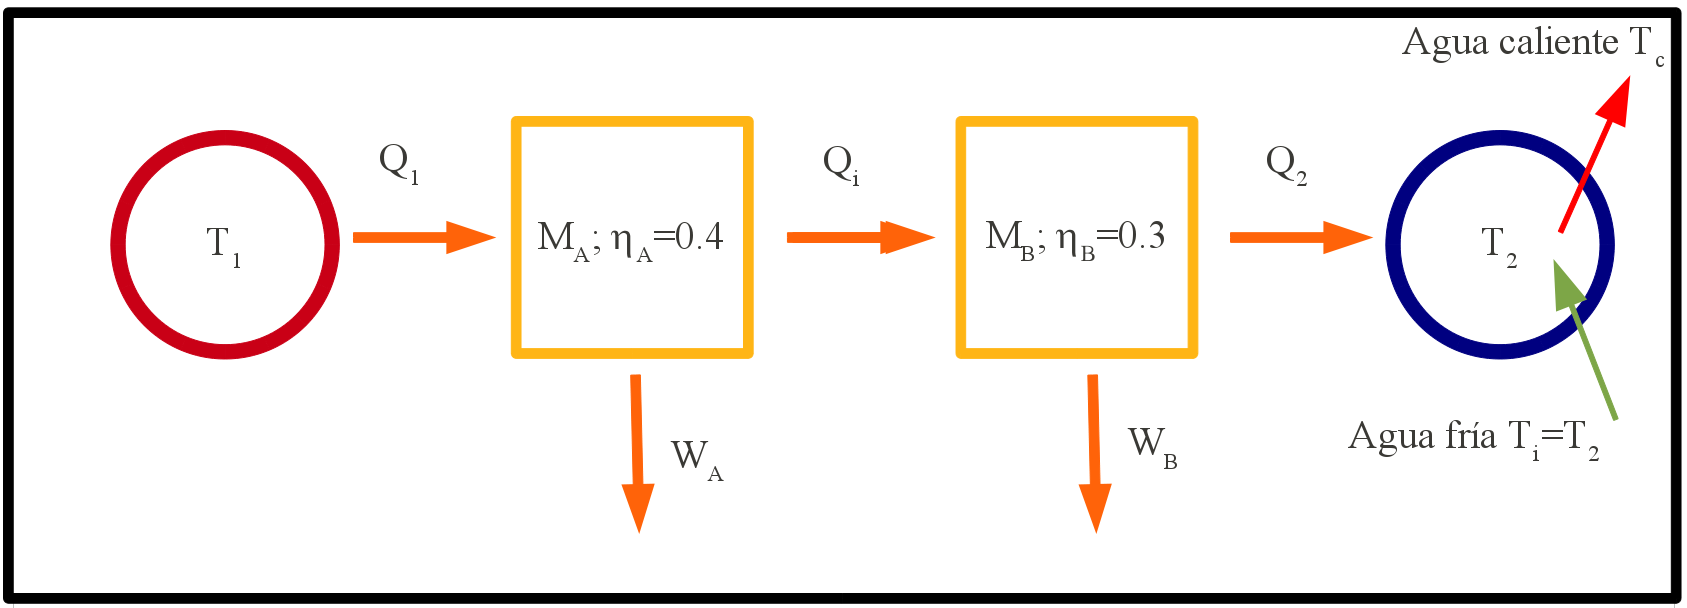
\includegraphics[width=0.9\textwidth]{maq2.png}
		\end{figure}
		\begin{enumerate}
			\item Calcule la cantidad de calor $Q_i$ que pasa de la máquina $A$
				a la $B$ cada segundo.
			\item Calcule el trabajo total producido: $W=W_A+W_B$ por segundo.
			\item Calcule la cantidad de calor $Q_2$ que pasa de la máquina $B$
				a la calefacción.
			\item Calcule el rendimiento total de la instalación de ciclo
				combinado, y diga cual es la ventaja de estas instalaciones.
			\item Compare el rendimiento anterior con el rendimiento de una
				máquina de Carnot operando entre esas temperaturas.
			\item Calcule cuantos litros de agua por segundo será posible
				calentar desde $T_2$ hasta $T_c$.
		\end{enumerate}
		{\bf{R}}: a) $Q_1=500$\,MJ; $Q_2=300$\,MJ. b) $W_{\mathrm{tot}}=290$\,MJ; c) $Q_2=210$\,MJ; d) $\eta=58\%$; e) $\eta_C=70.7\%$; f) $836$\,L/s
		
\end{enumerate}
\end{document}
%%%%
